%% Преамбула TeX-файла

% 1. Стиль и язык
\documentclass[utf8x, 14pt]{G7-32} % Стиль (по умолчанию будет 14pt)

% Остальные стандартные настройки убраны в preamble.inc.tex.
\sloppy

% Настройки стиля ГОСТ 7-32
% Для начала определяем, хотим мы или нет, чтобы рисунки и таблицы нумеровались в пределах раздела, или нам нужна сквозная нумерация.
\EqInChapter % формулы будут нумероваться в пределах раздела
\TableInChapter % таблицы будут нумероваться в пределах раздела
\PicInChapter % рисунки будут нумероваться в пределах раздела

% Добавляем гипертекстовое оглавление в PDF
\usepackage[
bookmarks=true, colorlinks=true, unicode=true,
urlcolor=black,linkcolor=black, anchorcolor=black,
citecolor=black, menucolor=black, filecolor=black,
]{hyperref}

\AfterHyperrefFix

% Альтернативный Пакет для создания списка терминов со ссылками на них
\usepackage{glossaries}
\usepackage[stylemods,style=long3col]{glossaries-extra}
\setabbreviationstyle[acronym]{long-short}
\makenoidxglossaries


\usepackage{microtype}% полезный пакет для микротипографии, увы под xelatex мало чего умеет, но под pdflatex хорошо улучшает читаемость

% Тире могут быть невидимы в Adobe Reader
\ifInvisibleDashes
\MakeDashesBold
\fi

\usepackage{graphicx}   % Пакет для включения рисунков

% С такими оно полями оно работает по-умолчанию:
% \RequirePackage[left=20mm,right=10mm,top=20mm,bottom=20mm,headsep=0pt,includefoot]{geometry}
% Если вас тошнит от поля в 10мм --- увеличивайте до 20-ти, ну и про переплёт не забывайте:
\geometry{right=20mm}
\geometry{left=30mm}
\geometry{bottom=20mm}
\geometry{ignorefoot}% считать от нижней границы текста


% Пакет Tikz
\usepackage{tikz}
\usetikzlibrary{arrows,positioning,shadows}

% Произвольная нумерация списков.
\usepackage{enumerate}

% ячейки в несколько строчек
\usepackage{multirow}

% itemize внутри tabular
\usepackage{paralist,array}

%\setlength{\parskip}{1ex plus0.5ex minus0.5ex} % разрыв между абзацами
\setlength{\parskip}{1ex} % разрыв между абзацами
\usepackage{blindtext}

% Центрирование подписей к плавающим окружениям
%\usepackage[justification=centering]{caption}

\usepackage{newfloat}
\DeclareFloatingEnvironment[
placement={!ht},
name=Equation
]{eqndescNoIndent}
\edef\fixEqndesc{\noexpand\setlength{\noexpand\parindent}{\the\parindent}\noexpand\setlength{\noexpand\parskip}{\the\parskip}}
\newenvironment{eqndesc}[1][!ht]{%
    \begin{eqndescNoIndent}[#1]%
\fixEqndesc%
}
{\end{eqndescNoIndent}}




\begin{document}
% Настройки листингов.
\ifPDFTeX
% % 8 Листинги

\usepackage{listings}

% Значения по умолчанию
\lstset{
  basicstyle= \footnotesize,
  breakatwhitespace=true,% разрыв строк только на whitespacce
  breaklines=true,       % переносить длинные строки
%   captionpos=b,          % подписи снизу -- вроде не надо
  inputencoding=koi8-r,
  numbers=left,          % нумерация слева
  numberstyle=\footnotesize,
  showspaces=false,      % показывать пробелы подчеркиваниями -- идиотизм 70-х годов
  showstringspaces=false,
  showtabs=false,        % и табы тоже
  stepnumber=1,
  tabsize=4,              % кому нужны табы по 8 символов?
  frame=single
}

% Стиль для псевдокода: строчки обычно короткие, поэтому размер шрифта побольше
\lstdefinestyle{pseudocode}{
  basicstyle=\small,
  keywordstyle=\color{black}\bfseries\underbar,
  language=Pseudocode,
  numberstyle=\footnotesize,
  commentstyle=\footnotesize\it
}

% Стиль для обычного кода: маленький шрифт
\lstdefinestyle{realcode}{
  basicstyle=\scriptsize,
  numberstyle=\footnotesize
}

% Стиль для коротких кусков обычного кода: средний шрифт
\lstdefinestyle{simplecode}{
  basicstyle=\footnotesize,
  numberstyle=\footnotesize
}

% Стиль для BNF
\lstdefinestyle{grammar}{
  basicstyle=\footnotesize,
  numberstyle=\footnotesize,
  stringstyle=\bfseries\ttfamily,
  language=BNF
}

% Определим свой язык для написания псевдокодов на основе Python
\lstdefinelanguage[]{Pseudocode}[]{Python}{
  morekeywords={each,empty,wait,do},% ключевые слова добавлять сюда
  morecomment=[s]{\{}{\}},% комменты {а-ля Pascal} смотрятся нагляднее
  literate=% а сюда добавлять операторы, которые хотите отображать как мат. символы
    {->}{\ensuremath{$\rightarrow$}~}2%
    {<-}{\ensuremath{$\leftarrow$}~}2%
    {:=}{\ensuremath{$\leftarrow$}~}2%
    {<--}{\ensuremath{$\Longleftarrow$}~}2%
}[keywords,comments]

% Свой язык для задания грамматик в BNF
\lstdefinelanguage[]{BNF}[]{}{
  morekeywords={},
  morecomment=[s]{@}{@},
  morestring=[b]",%
  literate=%
    {->}{\ensuremath{$\rightarrow$}~}2%
    {*}{\ensuremath{$^*$}~}2%
    {+}{\ensuremath{$^+$}~}2%
    {|}{\ensuremath{$|$}~}2%
}[keywords,comments,strings]

% Подписи к листингам на русском языке.
\renewcommand\lstlistingname{Листинг}
\renewcommand\lstlistlistingname{Листинги}

\else
\usepackage{local-minted}
\usepackage{lastpage}
\fi

% Полезные макросы листингов.
% Любимые команды
\newcommand{\Code}[1]{\textbf{#1}}


% Стиль титульного листа и заголовки

%\NirEkz{Экз. 3}                                  % Раскоментировать если не требуется
%\NirGrif{Секретно}                % Наименование грифа

%\gosttitle{Gost7-32}       % Шаблон титульной страницы, по умолчанию будет ГОСТ 7.32-2001, 
% Варианты GostRV15-110 или Gost7-32 
 
\NirOrgLongName{МИНОБРНАУКИ РОССИИ \\
% Российской Федерации\par
Федеральное государственное автономное образовательное учреждение высшего
образования
«Северо-Восточный федеральный университет имени М.К.Аммосова»
(СВФУ) \\
Инженерно-технический институт
}                                           %% Полное название организации

\NirUdk{УДК № 69}
% \NirGosNo{№ госрегистрации 01970006723}
%\NirInventarNo{Инв. № ??????}

%\NirConfirm{Согласовано}                  % Смена УТВЕРЖДАЮ
\NirBoss[.49]{Проректор по науке
и инновациям СВФУ}{Е.Э. Соловьев}            %% Заказчик, утверждающий НИР


%\NirReportName{Научно-технический отчет}   % Можно поменять тип отчета
%\NirAbout{О составной части \par опытно-конструкторской работы} %Можно изменить о чем отчет

%\NirPartNum{Часть}{1}                      % Часть номер

%\NirBareSubject{}                  % Убирает по теме если раскоментить

% \NirIsAnnotacion{АННОТАЦИОННЫЙ }         %% Раскомментируйте, если это аннотационный отчёт
%\NirStage{промежуточный}{Этап \No 1}{} %%% Этап НИР: {номер этапа}{вид отчёта - промежуточный или заключительный}{название этапа}
%\NirStage{}{}{} %%% Этап НИР: {номер этапа}{вид отчёта - промежуточный или 

\Nir{Разработка научно-обоснованных решений в проектировании, строительстве и
эксплуатации арктических поселений, отвечающих современным стандартам устойчивого
развития и комфортности проживания. Этап 1}

\NirSubject{Обзор и оценка решений по строительству и градостроительных принципов в условиях Арктики}                                   % Наименование темы
%\NirFinal{}                        % Заключительный, если закоментировать то промежуточный
%\finalname{итоговый}               % Название финального отчета (Заключительный) 
%\NirCode{Шифр\,---\,САПР-РЛС-ФИЗТЕХ-1} % Можно задать шифр как в ГОСТ 15.110
\NirCode{Шифр темы: ГК № 8019}

\NirManager{Руководитель темы, \\ Директор ИТИ, д.т.н., доцент}{Т.А. Корнилов  } %% Название руководителя
\NirIsp{Ответственный исполнитель, Менеджер УМО ИТИ, к.т.н.}{А.Л. Попов} %% Название руководителя

\NirYear{2022}%% если нужно поменять год отчёта; если закомментировано, ставится текущий год
\NirTown{Якутск, }                           %% город, в котором написан отчёт




\frontmatter % выключает нумерацию ВСЕГО; здесь начинаются ненумерованные главы: реферат, введение, глоссарий, сокращения и прочее.

\maketitle %создает титульную страницу


\begin{executors}
\personalSignature{Первый исполнитель}{ФИО}

\personalSignature{Второй исполнитель}{ФИО}
\end{executors}

%\listoffigures                         % Список рисунков

%\listoftables                          % Список таблиц

%\NormRefs % Нормативные ссылки 
% Команды \breakingbeforechapters и \nonbreakingbeforechapters
% управляют разрывом страницы перед главами.
% По-умолчанию страница разрывается.

% \nobreakingbeforechapters
% \breakingbeforechapters

% % Также можно использовать \Referat, как в оригинале


\begin{abstract}

    Отчет содержит \pageref{LastPage}\,стр.%
    \ifnum \totfig >0
    , \totfig~рис.%
    \fi
    \ifnum \tottab >0
    , \tottab~табл.%
    \fi
    %
    \ifnum \totbib >0
    , \totbib~источн.%
    \fi
    %
    \ifnum \totapp >0
    , \totapp~прил.%
    \else
    .%
    \fi


    Это пример каркаса расчётно-пояснительной записки, желательный к использованию в РПЗ проекта по курсу РСОИ
    \nocite{*}.

    Данный опус, как и более новые версии этого документа, можно взять по адресу (\url{https://github.com/latex-g7-32/latex-g7-32}).

    Текст в документе носит совершенно абстрактный характер.

\end{abstract}

%%% Local Variables: 
%%% mode: latex
%%% TeX-master: "rpz"
%%% End: 


\tableofcontents

\printnomenclature % Автоматический список сокращений

% \Introduction

Целью работы является создание всякой всячины. Для достижения поставленной цели необходимо решить следующие задачи:

\begin{itemize}
\item проанализировать существующую всячину;
\item спроектировать свою, новую всячину;
\item изготовить всякую всячину;
\item проверить её работоспособность.
\end{itemize}

Проверяем как у нас работают сокращения, обозначения и определения "---
MAX, 
\Abbrev{MAX}{Maximum ""--- максимальное значение параметра}
API 
\Abbrev{API}{application programming interface ""--- внешний интерфейс взаимодействия с приложением}
с обратным прокси.
\Define{Обратный прокси}{тип прокси-сервера, который ретранслирует}





\mainmatter % это включает нумерацию глав и секций в документе ниже

% \chapter{Аналитический раздел}
\label{cha:analysis}
%
% % В начале раздела  можно напомнить его цель
%
В данном разделе анализируется и классифицируется существующая всячина и пути создания новой всячины. А вот отступ справа в 1 см. "--- это хоть и по ГОСТ, но ведь диагноз же...

\section{Анализ того и сего}

% Обратите внимание, что включается не ../dia/..., а inc/dia/...
% В Makefile есть соответствующее правило для inc/dia/*.pdf, которое
% берет исходные файлы из ../dia в этом случае.

\begin{figure}
  \centering
  \includegraphics[width=\textwidth]{assets/figures/image (1)}
  \caption{Рисунок}
  \label{fig:fig01}
\end{figure}

\begin{figure}
  \centering
  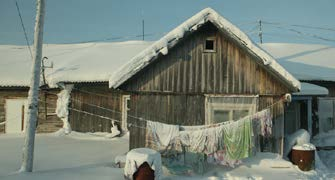
\includegraphics[width=\textwidth]{assets/figures/image}
  \caption{Рисунок}
  \label{fig:fig02}
\end{figure}

\begin{figure}
  \centering
  \includegraphics[height=0.85\textheight]{inc/img/leonardo}
  \caption{Предполагаемый автопортрет Леонардо да Винчи}
  \label{fig:leonardo}
\end{figure}

В \cite{wiki:latex} указано, что... \cite{Pup09}

Кстати, про картинки. Во-первых, для фигур следует использовать \texttt{[ht]}. Если и после этого картинки вставляются <<не по ГОСТ>>, т.е. слишком далеко от места ссылки, "--- значит у вас в РПЗ \textbf{слишком мало текста}! Хотя и ужасный параметр \texttt{!ht} у окружения \texttt{figure} тоже никто не отменял, только при его использовании документ получается страшный, как в ворде, поэтому просьба так не делать по возможности.

\section{Существующие подходы к созданию всячины}

Известны следующие подходы...

\begin{enumerate}
\item Перечисление с номерами.
\item Номера первого уровня. Да, ГОСТ требует именно так "--- сначала буквы, на втором уровне "--- цифры.
Чуть ниже будет вариант <<нормальной>> нумерации и советы по её изменению.
Да, мне так нравится: на первом уровне выравнивание элементов как у обычных абзацев. Проверим теперь вложенные списки.
\begin{enumerate}
\item Номера второго уровня.
\item Номера второго уровня. Проверяем на длииииной-предлиииииииииинной строке, что получается.... Сойдёт.
\end{enumerate}
\item По мнению Лукьяненко, человеческий мозг старается подвести любую проблему к выбору
  из трех вариантов.
\item Четвёртый (и последний) элемент списка.
\end{enumerate}

Теперь мы покажем, как изменить нумерацию на «нормальную», если вам этого захочется. Пара команд в начале документа поможет нам.

\renewcommand{\labelenumi}{\arabic{enumi})}
\renewcommand{\labelenumii}{\asbuk{enumii})}

\begin{enumerate}
\item Изменим нумерацию на более привычную...
\item ... нарушим этим гост.
\begin{enumerate}
\item Но, пожалуй, так лучше.
\end{enumerate}
\end{enumerate}

В заключение покажем произвольные маркеры в списках. Для них нужен пакет \textbf{enumerate}.
\begin{enumerate}[1.]
\item Маркер с арабской цифрой и с точкой.
\item Маркер с арабской цифрой и с точкой.
\begin{enumerate}[I.]
\item Римская цифра с точкой.
\item Римская цифра с точкой.
\end{enumerate}
\end{enumerate}

В отчётах могут быть и таблицы "--- см. табл.~\ref{tab:tabular} и~\ref{tab:longtable}.
Небольшая таблица делается при помощи \Code{tabular} внутри \Code{table} (последний
полностью аналогичен \Code{figure}, но добавляет другую подпись).

\begin{table}[ht]
  \caption{Пример короткой таблицы с коротким названием}
  \begin{tabular}{|r|c|c|c|l|}
  \hline
  Тело      & $F$ & $V$  & $E$ & $F+V-E-2$ \\
  \hline
  Тетраэдр  & 4   & 4    & 6   & 0         \\
  Куб       & 6   & 8    & 12  & 0         \\
  Октаэдр   & 8   & 6    & 12  & 0         \\
  Додекаэдр & 20  & 12   & 30  & 0         \\
  Икосаэдр  & 12  & 20   & 30  & 0         \\
  \hline
  Эйлер     & 666 & 9000 & 42  & $+\infty$ \\
  \hline
  \end{tabular}
  \label{tab:tabular}
\end{table}

Для больших таблиц следует использовать пакет \Code{longtable}, позволяющий создавать
таблицы на несколько страниц по ГОСТ.

Для того, чтобы длинный текст разбивался на много строк в пределах одной ячейки, надо в
качестве ее формата задавать \texttt{p} и указывать явно ширину: в мм/дюймах
(\texttt{110mm}), относительно ширины страницы (\texttt{0.22\textbackslash textwidth})
и~т.п.

Можно также использовать уменьшенный шрифт "--- но, пожалуйста, тогда уж во \textbf{всей}
таблице сразу.

\begin{center}
  \begin{longtable}{|p{0.40\textwidth}|c|p{0.30\textwidth}|}
    \caption{Пример длинной таблицы с длинным названием на много длинных-длинных строк}
    \label{tab:longtable}
    \\ \hline
    Вид шума & Громкость, дБ & Комментарий \\
    \hline \endfirsthead
    \subcaption{Продолжение таблицы~\ref{tab:longtable}}
    \\ \hline \endhead
    \hline \subcaption{Продолжение на след. стр.}
    \endfoot
    \hline \endlastfoot
    Порог слышимости             & 0     &                                                \\
    \hline
    Шепот в тихой библиотеке     & 30    &                                                \\
    Обычный разговор             & 60-70 &                                                \\
    Звонок телефона              & 80    & \small{Конечно, это было до эпохи мобильников} \\
    Уличный шум                  & 85    & \small{(внутри машины)}                        \\
    Гудок поезда                 & 90    &                                                \\
    Шум электрички               & 95    &                                                \\
    \hline
    Порог здоровой нормы         & 90-95 & \small{Длительное пребывание на более
    громком шуме может привести к ухудшению слуха}                                        \\
    \hline
    Мотоцикл                     & 100   &                                                \\
    Power Mower                  & 107   & \small{(модель бензокосилки)}                  \\
    Бензопила                    & 110   & \small{(Doom в целом вреден для здоровья)}     \\
    Рок-концерт                  & 115   &                                                \\
    \hline
    Порог боли                   & 125   & \small{feel the pain}                          \\
    \hline
    Клепальный молоток           & 125   & \small{(автор сам не знает, что это)}          \\
    \hline
    Порог опасности              & 140   & \small{Даже кратковременное пребывание на
    шуме большего уровня может привести к необратимым последствиям}                       \\
    \hline
    Реактивный двигатель         & 140   &                                                \\
                                 & 180   & \small{Необратимое полное повреждение
                                 слуховых органов}                                        \\
    Самый громкий возможный звук & 194   & \small{Интересно, почему?..}                   \\
  \end{longtable}
\end{center}

%%% Local Variables:
%%% mode: latex
%%% TeX-master: "rpz"
%%% End:

% \chapter{Конструкторский раздел}
\label{cha:design}

В данном разделе проектируется новая всячина.

\section{Архитектура всячины}

\subsection{Протестируем подпункт}
\subsubsection{А теперь подподпункт}


\paragraph{Проверка} параграфа. Вроде работает.
\paragraph{Вторая проверка} параграфа. Опять работает.

Вот.

\begin{itemize}
\item Это список с <<палочками>>.
\item Хотя он и по ГОСТ, но\dots
\end{itemize}

\begin{enumerate}
\item  Для списка, начинающегося с заглавной буквы, лучше список с цифрами.
\end{enumerate}

Формула \eqref{F:F1} совершено бессмысленна.

%Кстати, при каких-то условиях <<удавалось>> получить двойный скобки вокруг номеров формул. Вопрос исследуется.

\begin{equation}
a= cb
\label{F:F1}
\end{equation}

А формула~\eqref{eq:fourierrow} имеет некоторый смысл.
Кроме этого она пытается иллюстрировать применение окружения \Code{eqndesc} которое размещает формулу совместно с её описанием.
Однако обратите внимание на нумерацию формул~\eqref{eq:fourierrow} и \eqref{F:F2}, попробуйте добавить \Code{[H]} к такой формуле.

\begin{eqndesc}
    \begin{equation}\label{eq:fourierrow}
        f(x) = \frac{a_0}{2} + \sum\limits_{k=1}^{+\infty} A_k\cos\left(k\frac{2\pi}{\tau}x+\theta_k\right)
    \end{equation}

    где $A_k$ "--- амплитуда  k-го гармонического колебания,\\
    $A_k$ "--- амплитуда $k$-го гармонического колебания,\\
    $ k\frac{2\pi}{\tau} = k\omega$ "--- круговая частота гармонического колебания,\\
    $\theta_k$ "--- начальная фаза $k$-го колебания.
\end{eqndesc}


Окружение \texttt{cases} опять работает (см. \eqref{F:F2}), спасибо И. Короткову за исправления..


\begin{equation}
a= \begin{cases}
 3x + 5y + z, \mbox{если хорошо} \\
 7x - 2y + 4z, \mbox{если плохо}\\
 -6x + 3y + 2z, \mbox{если совсем плохо}
\end{cases}
\label{F:F2}
\end{equation}

\section{Подсистема всякой ерунды}

Культурная вставка dot-файлов через утилиту dot2tex (рис.~\ref{fig:fig02}).

\begin{figure}
  \centering
% [width=0.5\textwidth] --- регулировка ширины картинки
  \includegraphics[width=.5\textwidth]{inc/dot/cow2}
  \caption{Рисунок}
  \label{fig:fig02}
\end{figure}


\subsection{Блок-схема всякой ерунды}

\subsubsection*{Кстати о заголовках}

У нас есть и \Code{subsubsection}. Только лучше её не нумеровать.

%%% Local Variables:
%%% mode: latex
%%% TeX-master: "rpz"
%%% End:

% \chapter{Технологический раздел}
\label{cha:impl}

В данном разделе описано изготовление и требование всячины. Кстати,
в Latex нужно эскейпить подчёркивание (писать <<\verb|some\_function|>> для \Code{some\_function}).

\ifPDFTeX
Для вставки кода есть пакет \Code{listings}. К сожалению, пакет \Code{listings} всё ещё
работает криво при появлении в листинге русских букв и кодировке исходников utf-8.
В данном примере он (увы) на лету конвертируется в koi-8 в ходе сборки pdf.

Есть альтернатива \Code{listingsutf8}, однако она работает лишь с
\Code{\textbackslash{}lstinputlisting}, но не с окружением \Code{\textbackslash{}lstlisting}

Вот так можно вставлять псевдокод (питоноподобный язык определен в \Code{listings.inc.tex}):

\begin{lstlisting}[style=pseudocode,caption={Алгоритм оценки дипломных работ}]
def EvaluateDiplomas():
    for each student in Masters:
        student.Mark := 5
    for each student in Engineers:
        if Good(student):
            student.Mark := 5
        else:
            student.Mark := 4
\end{lstlisting}

Еще в шаблоне определен псевдоязык для BNF:

\begin{lstlisting}[style=grammar,basicstyle=\small,caption={Грамматика}]
  ifstmt -> "if" "(" expression ")" stmt |
            "if" "(" expression ")" stmt1 "else" stmt2
  number -> digit digit*
\end{lstlisting}

В листинге~\ref{lst:sample01} работают русские буквы. Сильная магия. Однако, работает
только во включаемых файлах, прямо в \TeX{} нельзя.

% Обратите внимание, что включается не ../src/..., а inc/src/...
% В Makefile есть соответствующее правило для inc/src/*,
% которое копирует исходные файлы из ../src и конвертирует из UTF-8 в KOI8-R.
% Кстати, поэтому использовать можно только русские буквы и ASCII,
% весь остальной UTF-8 вроде CJK и египетских иероглифов -- нельзя.

\lstinputlisting[language=C,caption=Пример (\Code{test.c}),label=lst:sample01]{inc/src/test.c}

\else

Для вставки кода есть пакет \texttt{minted}. Он хорош всем кроме: необходимости Python (есть во всех нормальных (нет, Windows, я не про тебя) ОС) и Pygments и того, что нормально работает лишь в \XeLaTeX.

\ifdefined\NoMinted
Но к сожалению, у вас, по-видимому, не установлен Python или pygmentize.
\else
Можно пользоваться расширенным BFN:

\begin{listing}[H]
\begin{ebnfcode}
 letter = "A" | "B" | "C" | "D" | "E" | "F" | "G"
       | "H" | "I" | "J" | "K" | "L" | "M" | "N"
       | "O" | "P" | "Q" | "R" | "S" | "T" | "U"
       | "V" | "W" | "X" | "Y" | "Z" ;
digit = "0" | "1" | "2" | "3" | "4" | "5" | "6" | "7" | "8" | "9" ;
symbol = "[" | "]" | "{" | "}" | "(" | ")" | "<" | ">"
       | "'" | '"' | "=" | "|" | "." | "," | ";" ;
character = letter | digit | symbol | "_" ;
 
identifier = letter , { letter | digit | "_" } ;
terminal = "'" , character , { character } , "'" 
         | '"' , character , { character } , '"' ;
 
lhs = identifier ;
rhs = identifier
     | terminal
     | "[" , rhs , "]"
     | "{" , rhs , "}"
     | "(" , rhs , ")"
     | rhs , "|" , rhs
     | rhs , "," , rhs ;
 
rule = lhs , "=" , rhs , ";" ;
grammar = { rule } ;
\end{ebnfcode}
\caption{EBNF определённый через EBNF}
\label{lst:ebnf}
\end{listing}

А вот в листинге \ref{lst:c} на языке C работают русские комменты. Спасибо Pygments и Minted за это.

\begin{listing}[H]
\cfile{inc/src/test.c}
\caption{Пример — test.c} 
\end{listing}
\label{lst:c}

\fi
\fi
% Для вставки реального кода лучше использовать \texttt{\textbackslash lstinputlisting} (который понимает
% UTF8) и стили \Code{realcode} либо \Code{simplecode} (в зависимости от размера куска).




Можно также использовать окружение \Code{verbatim}, если \Code{listings} чем-то не
устраивает. Только следует помнить, что табы в нём <<съедаются>>. Существует так же команда \Code{\textbackslash{}verbatiminput} для вставки файла.

\begin{verbatim}
a_b = a + b; // русский комментарий
if (a_b > 0)
    a_b = 0;
\end{verbatim}

%%% Local Variables:
%%% mode: latex
%%% TeX-master: "rpz"
%%% End:

% \chapter{Экспериментальный раздел}
\label{cha:research}

В данном разделе проводятся вычислительные эксперименты.
А на рис.~\ref{fig:spire01} показана схема мыслительного процесса автора...

\begin{figure}
  \centering
  \includegraphics[width=\textwidth]{inc/svg/pic01}
  \caption{Как страшно жить}
  \label{fig:spire01}
\end{figure}


%%% Local Variables:
%%% mode: latex
%%% TeX-master: "rpz"
%%% End:

% \chapter{Организационно-экономический раздел}
\label{cha:econom}

\section{Протестируем специальные символы.}

И заодно переключение шрифтов.


{\shorthandoff" \texttt{"-{}-* Прямая речь "-{}-{}- <{}<после ,{},тире`{}` неразрывный пробел>{}>}}

{\cyrillicfonttt{\bfseries\itshape\textbackslash{}cyrillicfonttt}
"--* Прямая речь "--- <<после ,,тире`` неразрывный пробел>>.}

{\cyrillicfontsf{\bfseries\itshape\textbackslash{}cyrillicfontsf}
"--* Прямая речь "--- <<после ,,тире`` неразрывный пробел>>.}

{\cyrillicfont{\bfseries\itshape\textbackslash{}cyrillicfont}
"--* Прямая речь "--- <<после ,,тире`` неразрывный пробел>>.}


\blindtext
%%% Local Variables:
%%% mode: latex
%%% TeX-master: "rpz"
%%% End:

% \chapter{Промышленная экология и безопасность}\label{cha:bzd}

\blindtext

\blindlistlist[3]{enumerate}

%%% Local Variables:
%%% mode: latex
%%% TeX-master: "rpz"
%%% End:


\chapter{Обзор и оценка градостроительных принципов и способов реализации жилищного строительства в условиях Арктики}
В главе авторы рассматривают способы выживания и расселения, сформированные коренным населением Арктики.
Производится обощение опыта и выявление наиболее востребованных практик, применимых при градостроительном планировании и принятии решений,
на основе сравнения опыта организации расселения коренного населения с современными практиками управления территориями, на следующих уровнях:
\begin{enumerate}[1)]
    \item государственном (федеральном) — уровень принятия решений высшего руководства страны и подведомственных правительству организации — министерств, ведомств, надзорных органов и др.;
    \item региональном (субъекта) — уровень принятия решений на территории государства, для которой законодательством этого государства определены принципы организации самоуправления;
    \item общинном — уровень принятия решений сообществ, товариществ собственников, гильдий и аналогичных схожих по организационной форме
    социальных образований, действующих на основании устава или общей общественной идеи;
    \item частного домохозяйства (частном) — уровень принятия решения отдельной ячейки общества — семьи, индивида и др., распоряжающихся частным
    домохозяйством, собственными материальными ресурсами и капиталом.
\end{enumerate}
Цитата по \footnote{см. \cite{up_Avdotin_GradProektirovanie,law_RU_GradoCodex,nomads_Golovnev_NomadsTechAtlas}}


% Сниски \footnote[8]{Восьмая}
% или вусё же сноски \footnote[]{Восьмая}


\section{Традиционные подходы в организации жилища и адаптация к условиям Арктики}\label{CH01_experience_indigenous}
Объективную оценку степени экстремальности, <<суровости>>, окружающей среды возможно произвести по нескольким показателям, среди которых авторы выделяют:

\begin{itemize}
    \item продолжительность отопительного периода, выражаемое в градус-сутках отопительного периода (ГСОП);
    \item наличие доступа к пригодной для питья воды, выражаемое в м³/км расстояния до источника;
    \item наличие и доступность пригодного для дыхания кислорода, выражаемое в м³/час;
    \item стоимости доставки грузов, у.е./км;
    \item продолжительность естественной освещённости, выражаемая в часах;
\end{itemize}


Традиционные, выработанные веками коренным (местным) населением объемно-планировочные решения в строительстве жилища и хозяйственных построек,
продиктованных проживанием в экстремальных природно-климатических условиях Арктики, направлены на адаптацию к таковым условиям.

Коренные жители арктических районов в основу быта преимущественно ставили скотоводство, основанное на разведении оленей, береговые поселенцы, такие как чукчи,
эскимосы и коряки практиковали также морской зверобойный промысел. Оленеводам был свойственен кочевой образ жизни, причем перемещались они по определенным традиционно
складывающимся маршрутам каслания (выпаса стада на протяжении сезона) оленей, которые мигрировали по мере поедания растущего на пастбищах ягеля. Селения-стойбища оленеводов
могли обустраиваться на новых местах с периодичностью в несколько дней или недель. При этом некоторые народы использовали переносные жилища, другие же --– передвижные, называемые также балками (Рис.~\ref{fig:ch01_s10_urbanplan_settelsystems03}) [170, с. 9].

Представители коренных этносов имели ясное представление о гепатогенных областях, и прежде чем где-либо селиться тщательно узнавали о местных условиях,
анализировали происходящие природные явления [172, с. 76]. Стойбища, как правило, размещали в определенных местах.
Летом выбирали участки на возвышенностях у воды в обдуваемом ветрами месте, чтобы гнус не беспокоил стада оленей.
Зимой же, наоборот, стойбища располагали в безветренных лощинах, а также рядом с растительностью, служащей топливом и преградой от ветров и метелей.
Чумы оленеводы ставили на довольно большом расстоянии друг от друга, иногда доходящем до 10 метров и более, группируя их по 2-3 штуки.
Стойбища ненцев состояли из 1-3 чумом, летом же они могли сооружать до десяти чумов в одном месте. Для стойбищ чукчей была характерна постановка от 2 до 10 яранг, а для эскимосов уже от 10-15 до 20-50 яранг.
Конфигурация расположения жилищ у разных народов была своя: так, эвены, при достаточно большом количестве чумов, располагали их по кругу, если же их число небольшое – то ставили полукругом (рисунок 74, приложение А.4). Чукчи размещали яранги линейно в направлении с востока на запад [158, с. 458].

На некотором расстоянии от чума, автохтоны подготавливали место для организации костра. Справа и слева от чумов ставили нарты с имуществом и продуктовыми запасами.
Иногда в целях хранения продуктов питания возводили специальные навесы или же помосты на столбах [170, с. 10].

\begin{figure}
    \centering
    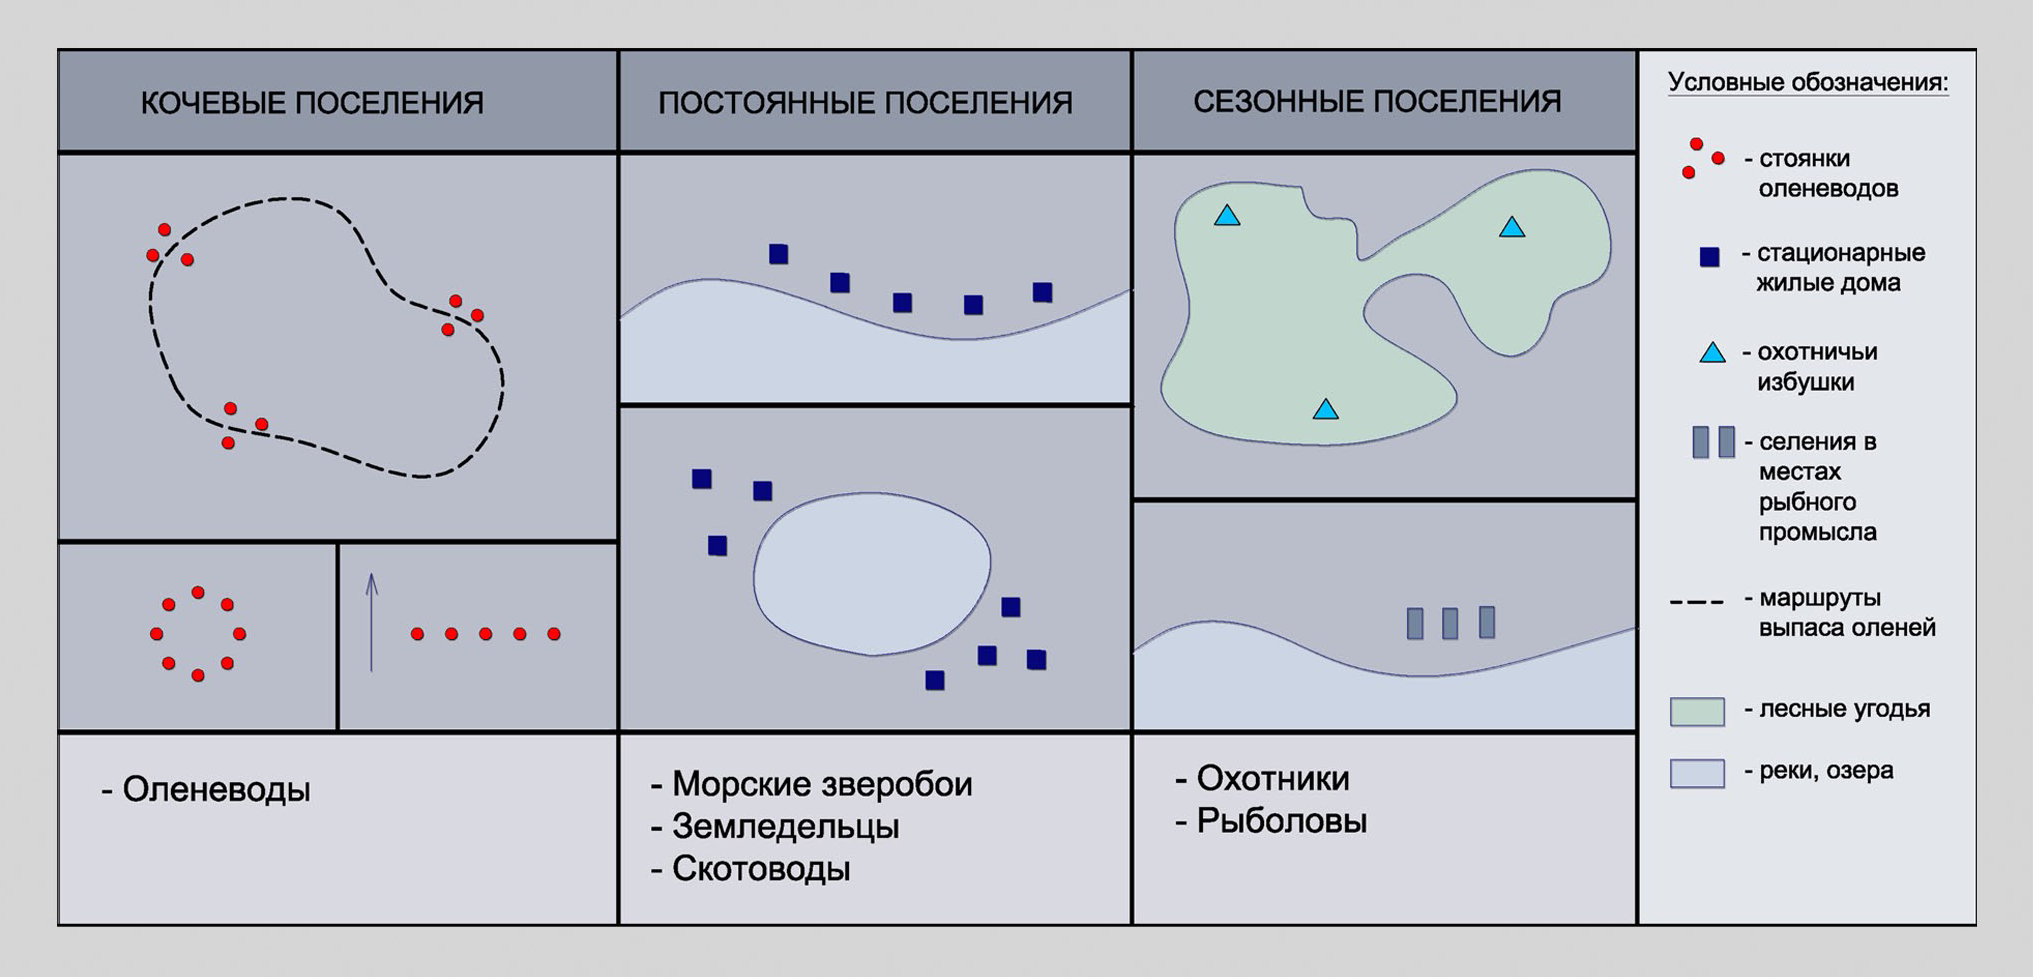
\includegraphics[width=\textwidth]{assets/figures/ch01_s10_urbanplan_settelsystems03}
    \caption{Типы традиционных поселений коренных народов Севера (графика разработана Благодетелевой О.М.)}
    \author{графика разработана Благодетелевой О.М.}
    \label{fig:ch01_s10_urbanplan_settelsystems03}
  \end{figure}

\gls{api}

% \glsxtrfull{api} % вызов полной формы термина в тексте

\gls{coolt}

\gls{coolt}

\include{abr_CH01_experience_goverments}
\include{abr_CH01_conclusion}

\backmatter %% Здесь заканчивается нумерованная часть документа и начинаются ссылки и
            
\Conclusion % заключение к отчёту

В результате проделанной работы стало ясно, что ничего не ясно...

%%% Local Variables: 
%%% mode: latex
%%% TeX-master: "rpz"
%%% End: 
%% заключение


% % Список литературы при помощи BibTeX
% Юзать так:
%
% pdflatex rpz
% bibtex rpz
% pdflatex rpz

\bibliographystyle{./BibTeX-Styles/ugost2003s}
% Подключить библиографию из каталога ./bibliography/2022/...
\bibliography{
    ./bibliography/2022/common_laws,
    ./bibliography/2022/research_arcticbuildtech_sciAndResearches,
    ./bibliography/2022/research_arcticbuildtech_urbanPlanningTexts
}

%%% Local Variables: 
%%% mode: latex
%%% TeX-master: "rpz"
%%% End: 



\appendix   % Тут идут приложения

% \chapter{Картинки}
\label{cha:appendix1}

\blindtext
\begin{figure}
\centering
\caption{Картинка в приложении. Страшная и ужасная.}
\end{figure}

%%% Local Variables: 
%%% mode: latex
%%% TeX-master: "rpz"
%%% End: 


% \chapter{Еще картинки}
\label{cha:appendix2}
\blindtext

\begin{figure}
\centering
\caption{Еще одна картинка, ничем не лучше предыдущей. Но надо же как-то заполнить место.}
\end{figure}

%%% Local Variables: 
%%% mode: latex
%%% TeX-master: "rpz"
%%% End: 


\end{document}

%%% Local Variables:
%%% mode: latex
%%% TeX-master: t
%%% End:
